\subsection{Entity-Relationship Schema} 

The following ER schema contains six entities which are going to be described in details in this section.\\ \\

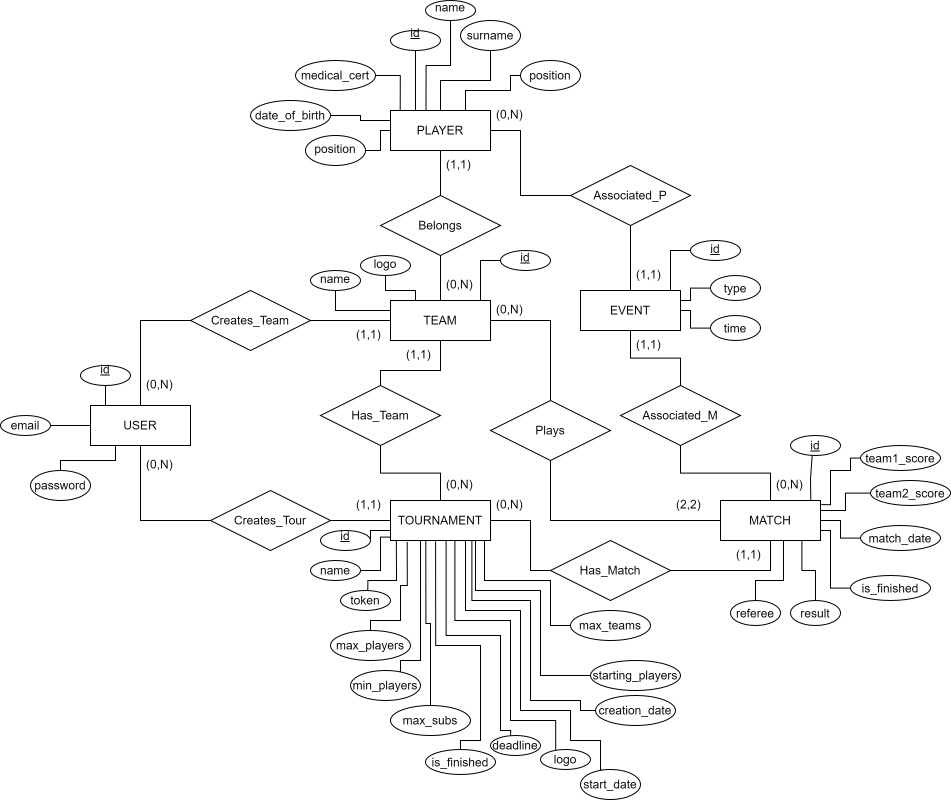
\includegraphics[scale = 0.50]{sections/DLL/ERSchema.png}\\
\newpage

\begin{enumerate}
    \item \textbf{User:} Entity Type User contains ID (INT), Email (CHAR) and Password (CHAR) for every user. The primary key is ID, while Email is a unique column. Every user can create one or more tournaments as well as one or more teams.
    
    \item \textbf{Tournament:} Entity Type Tournament contains ID (INT), Name (CHAR), Token (CHAR), Creator\_User\_ID (INT), Max\_Teams (INT), Max\_Players (INT), Min\_Players (INT), Starting\_Players (INT), Max\_Substitutions (INT), Deadline (DATETIME), Start\_Date (DATETIME), Creation\_Date (DATETIME), Logo (CHAR) and Is\_Finished (BOOL). The primary key is ID, Name is a unique column while Creator\_User\_ID is a foreign key constraint to the User table. Logo contains path to the file which represents logo for a particular tournament. Max\_Players and Min\_Players are maximum and minimum numbers of players for each team in the tournament, while Starting\_Players is a number of players in each match of the tournament and defines the type of tournament that is being organized (football, futsal etc.). Deadline represents the date until which teams can be enrolled. Starting\_Date is the date of the first match, while Creation\_Date indicates the date of the creation of the tournament. Is\_Finished indicates whether a tournaments is over or not. Each tournament must be created by exactly one user and has zero or more teams and matches.
    
    \item \textbf{Team:} Entity Type Team contains ID (INT), Name (CHAR), Logo (CHAR), Creator\_User\_ID (INT) and Tournament\_ID (INT). The primary key is ID, Name is a unique column while Creator\_User\_ID is a foreign key constraint to the User table and Tournament\_ID is a foreign key constraint to the Tournament table. Every Team must belong to exactly one tournament and must be created by a user. This Entity Type can have multiple players and can play multiple matches. 

    \item \textbf{Player:} Entity Type Player contains ID (INT), Name (CHAR), Surname (CHAR), Team\_ID (INT), Position (ENUM), Medical\_Certificate (CHAR) and Date\_Of\_Birth (DATETIME). The primary key is ID while Team\_ID is a foreign key constraint to the Team table.  Medical\_Certificate contains path to the file which represents Medical Certificate for a particular player. Every player must belong to a team and can be participant in more events.

    \item \textbf{Match:} Entity Type Match contains ID (INT), Team1\_ID (INT), Team2\_ID (INT), Tournament\_ID (INT), Team1\_Score (INT), Team2\_Score (INT), Result (CHAR), Referee (CHAR), Match\_Date (DATETIME) and Is\_Finished (BOOL). The primary key is ID while Team1\_ID and Team2\_ID are foreign keys constraint to the respective teams. Tournament\_ID is a foreign key constraint to the respective tournament. Every match must belong to only one tournament, have always two teams and can have multiple events associated to it.

    \item \textbf{Event:} Entity Type Event contains ID (INT), Match\_ID (INT), Player\_ID (INT), Type (Enum) and Time (DATETIME). The primary key is ID while Match\_ID is a foreign key constraint to the Match table and Player\_ID is a foreign key constraint to the Player table. Every event belongs to one match and has one Player who made the event. Type of event can be goal, yellow card or red card.
\end{enumerate}
